%%%%%%%%%%%%%%%%%%%%%%%%%%%%%%%%%%%%%%%%%%%%%%%%%%%%%%%%%%%%%%%%%%%%%%%%%%%%%%%%%%%%%%%%%%%%%%%%%%%%%%%%%%%%%%%%%%%%%%%%%%%%%%%%%%%%%%%%%%%%
%%%%%%%%%%%%%%%%%%%%%%%%%%%%%%%%%%%%%%%%%%%%%%%%%%%%% Start Of the Kicking Mechanism %%%%%%%%%%%%%%%%%%%%%%%%%%%%%%%%%%%%%%%%%%%%%%%%%%%%%%%
%%%%%%%%%%%%%%%%%%%%%%%%%%%%%%%%%%%%%%%%%%%%%%%%%%%%%%%%%%%%%%%%%%%%%%%%%%%%%%%%%%%%%%%%%%%%%%%%%%%%%%%%%%%%%%%%%%%%%%%%%%%%%%%%%%%%%%%%%%%%

\section{Kicking Mechanism}

%%%%%%%%%%%%%%%%%%%%%%%%%%%%%%%%%%%%%%%%%%%%%%%%%%%%%%%%%%%%%%%%%%%%%%%%%%%%%%%%%%%%%%%%%%%%%%%%%%%%%%%%%%%%%%%%%%%%%%%%%%%%%%%%%%%%%%%%%%%%
%%%%%%%%%%%%%%%%%%%%%%%%%%%%%%%%%%%%%%%%%%%%%%%%%%%%% Start Of the Kicking Mechanism I %%%%%%%%%%%%%%%%%%%%%%%%%%%%%%%%%%%%%%%%%%%%%%%%%%%%%%%
%%%%%%%%%%%%%%%%%%%%%%%%%%%%%%%%%%%%%%%%%%%%%%%%%%%%%%%%%%%%%%%%%%%%%%%%%%%%%%%%%%%%%%%%%%%%%%%%%%%%%%%%%%%%%%%%%%%%%%%%%%%%%%%%%%%%%%%%%%%%
    \subsection{Mechanism I}
%%%%%%%%%%%%%%%%%%%%%%%%%%%%%%%%%%%%%%%%%%%%%%%%%%%%%%%%%%%%%%%%%%%%%%%%%%%%%%%%%%%%%%%%%%%%%%%%%%%%%%%%%%%%%%%%%%%%%%%%%%%%%%%%%%%%%%%%%%%%
%%%%%%%%%%%%%%%%%%%%%%%%%%%%%%%%%%%%%%%%%%%%%%%% Components Used in the Kicking Mechanism %%%%%%%%%%%%%%%%%%%%%%%%%%%%%%%%%%%%%%%%%%%%%%%%%%
%%%%%%%%%%%%%%%%%%%%%%%%%%%%%%%%%%%%%%%%%%%%%%%%%%%%%%%%%%%%%%%%%%%%%%%%%%%%%%%%%%%%%%%%%%%%%%%%%%%%%%%%%%%%%%%%%%%%%%%%%%%%%%%%%%%%%%%%%%%%
        \subsubsection{Components Used}

        \begin{table}[h]

            \caption {Actuators Used on PR} \label{Actuators_K}  \small
            \begin{tabular}{|c|l|l|l|}
                \hline  \hline
                \textbf{Sr No}  & \textbf{Name Of the Component}& \textbf{Specifications}               & \textbf{Usage}                                                   \\ \hline    \hline
                \textbf{1}      & \textbf{Rod End Bearing}      & \textbf{ID: 10 }mm                    & To accommodate the misalignment of the piston rod, rod end       \\
                                &                               &                                       & bearing is used. The shaft of the piston rod is placed           \\ 
                                &                               &                                       & in a ball swivel of bearing placed inside the outer casing.      \\ \hline
                \textbf{2}      & \textbf{Pneumatic }           & \textbf{300 mm} stroke length         & To provide angular travel and required force to thee             \\
                                & \textbf{Cylinder}             & \textbf{25 mm} bore diameter,         & hitting partof the mechanism.                                    \\ \hline 
                \textbf{3}      & \textbf{Direction Control}    & $\textbf{5/2}$ DCV                    & It is used for position control of the air cylinder at the       \\
                                & \textbf{Valve (DCV)}          &                                       & end and starting position only.                                  \\ \hline    \hline   
            \end{tabular}

        \end{table}
%%%%%%%%%%%%%%%%%%%%%%%%%%%%%%%%%%%%%%%%%%%%%%%%%%%%%%%%%%%%%%%%%%%%%%%%%%%%%%%%%%%%%%%%%%%%%%%%%%%%%%%%%%%%%%%%%%%%%%%%%%%%%%%%%%%%%%%%%%%%
%%%%%%%%%%%%%%%%%%%%%%%%%%%%%%%%%%%%%%%%%%%%%%%%%%%%%%%%%%%%%%%%%% End %%%%%%%%%%%%%%%%%%%%%%%%%%%%%%%%%%%%%%%%%%%%%%%%%%%%%%%%%%%%%%%%%%%%%
%%%%%%%%%%%%%%%%%%%%%%%%%%%%%%%%%%%%%%%%%%%%%%%%%%%%%%%%%%%%%%%%%%%%%%%%%%%%%%%%%%%%%%%%%%%%%%%%%%%%%%%%%%%%%%%%%%%%%%%%%%%%%%%%%%%%%%%%%%%% 


%%%%%%%%%%%%%%%%%%%%%%%%%%%%%%%%%%%%%%%%%%%%%%%%%%%%%%%%%%%%%%%%%%%%%%%%%%%%%%%%%%%%%%%%%%%%%%%%%%%%%%%%%%%%%%%%%%%%%%%%%%%%%%%%%%%%%%%%%%%%
%%%%%%%%%%%%%%%%%%%%%%%%%%%%%%%%%%%%%%%%%%%%%% Start Of Principle Involved in the Mechanism %%%%%%%%%%%%%%%%%%%%%%%%%%%%%%%%%%%%%%%%%%%%%%%%
%%%%%%%%%%%%%%%%%%%%%%%%%%%%%%%%%%%%%%%%%%%%%%%%%%%%%%%%%%%%%%%%%%%%%%%%%%%%%%%%%%%%%%%%%%%%%%%%%%%%%%%%%%%%%%%%%%%%%%%%%%%%%%%%%%%%%%%%%%%%
        \subsubsection{Principle Involved in the mechanism}
            The kinetic energy of piston of air cylinder along with the potential energy of kicking link is converted
            into rotational energy of kicking link which is finally converted to the kinetic energy of the ball.
%%%%%%%%%%%%%%%%%%%%%%%%%%%%%%%%%%%%%%%%%%%%%%%%%%%%%%%%%%%%%%%%%%%%%%%%%%%%%%%%%%%%%%%%%%%%%%%%%%%%%%%%%%%%%%%%%%%%%%%%%%%%%%%%%%%%%%%%%%%%
%%%%%%%%%%%%%%%%%%%%%%%%%%%%%%%%%%%%%%%%%%%%%%%%%%%%%%%%%%%%%%%%%% End %%%%%%%%%%%%%%%%%%%%%%%%%%%%%%%%%%%%%%%%%%%%%%%%%%%%%%%%%%%%%%%%%%%%%
%%%%%%%%%%%%%%%%%%%%%%%%%%%%%%%%%%%%%%%%%%%%%%%%%%%%%%%%%%%%%%%%%%%%%%%%%%%%%%%%%%%%%%%%%%%%%%%%%%%%%%%%%%%%%%%%%%%%%%%%%%%%%%%%%%%%%%%%%%%% 

%%%%%%%%%%%%%%%%%%%%%%%%%%%%%%%%%%%%%%%%%%%%%%%%%%%%%%%%%%%%%%%%%%%%%%%%%%%%%%%%%%%%%%%%%%%%%%%%%%%%%%%%%%%%%%%%%%%%%%%%%%%%%%%%%%%%%%%%%%%%
%%%%%%%%%%%%%%%%%%%%%%%%%%%%%%%%%%%%%%%%%%%%%%%% Design Calculation of the Piston Kicking %%%%%%%%%%%%%%%%%%%%%%%%%%%%%%%%%%%%%%%%%%%%%%%%%%
%%%%%%%%%%%%%%%%%%%%%%%%%%%%%%%%%%%%%%%%%%%%%%%%%%%%%%%%%%%%%%%%%%%%%%%%%%%%%%%%%%%%%%%%%%%%%%%%%%%%%%%%%%%%%%%%%%%%%%%%%%%%%%%%%%%%%%%%%%%%
        \subsubsection{Design Calculations}
            o The calculation for angular travel of the hitting part of mechanism actuated using pneumatic air cylinder (Fig 3).                    \\
            o In angular travel calculation, we are tracingan arc travelled by rod end bearing at the endpoint ofthe piston rod.                    \\
                \textbf{A:} Initial position of the endpoint of the piston rod.                                                                     \\
                \textbf{B:} The endpoint of the piston rod.                                                                                         \\
                \textbf{C:} The pivot point of kicking link.                                                                                        \\
                \textbf{D:} The pivot point of an air cylinder.                                                                                     \\
            o Steps in calculations and deciding the height of pivot for air cylinder and the distance between 2 pivots:                            \\
                \textbf{1.} Considering the length of the kicking part, an arc is drawn with centre at c with some clearance from the ground.       \\
                \textbf{2.} For a given cylinder, $\textbf{90\degree}$ angular travel of the hitting part is preferred to impart maximum force and velocity 
                            to the kickball. \textbf{Angular travel more than 90 0 is not preferred since for that particular angle, piston 
                            motion inside air cylinder is restricted.}                                                                                  \\
                \textbf{3.} A vertical line passing through centre C is drawn, ensuring a $\textbf{30\degree}$ angle in forwarding \textbf{((B)} and
                            a $\textbf{60\degree}$ angle in the backward direction \textbf{(ponit A)}.                                                  \\    
                \textbf{4.} Considering the retracted position of the piston of the air cylinder, an arc taking \textbf{(A} as a centre with
                            the length of retracted position (425 mm) is drawn. Again, extended length (725 mm) of the piston in air cylinder
                            is taken into consideration to draw an arc with centre at B. The point of intersection of these 2 is point D which
                            is actually the pivot point of the air cylinder.                                                                            \\
    
%%%%%%%%%%%%%%%%%%%%%%%%%%%%%%%%%%%%%%%%%%%%%%%%%%%%%%%%%%%%%%%%%%%%%%%%%%%%%%%%%%%%%%%%%%%%%%%%%%%%%%%%%%%%%%%%%%%%%%%%%%%%%%%%%%%%%%%%%%%%
%%%%%%%%%%%%%%%%%%%%%%%%%%%%%%%%%%%%%%%%%%%%%%%%%%%%%%%%%%%%%%%%%% End %%%%%%%%%%%%%%%%%%%%%%%%%%%%%%%%%%%%%%%%%%%%%%%%%%%%%%%%%%%%%%%%%%%%%
%%%%%%%%%%%%%%%%%%%%%%%%%%%%%%%%%%%%%%%%%%%%%%%%%%%%%%%%%%%%%%%%%%%%%%%%%%%%%%%%%%%%%%%%%%%%%%%%%%%%%%%%%%%%%%%%%%%%%%%%%%%%%%%%%%%%%%%%%%%% 


%%%%%%%%%%%%%%%%%%%%%%%%%%%%%%%%%%%%%%%%%%%%%%%%%%%%%%%%%%%%%%%%%%%%%%%%%%%%%%%%%%%%%%%%%%%%%%%%%%%%%%%%%%%%%%%%%%%%%%%%%%%%%%%%%%%%%%%%%%%%%%
%%%%%%%%%%%%%%%%%%%%%%%%%%%%%%%%%%%%%%%%%%%%%%%%%%%% Working of the Kicking Mechanism I %%%%%%%%%%%%%%%%%%%%%%%%%%%%%%%%%%%%%%%%%%%%%%%%%%%%%%
%%%%%%%%%%%%%%%%%%%%%%%%%%%%%%%%%%%%%%%%%%%%%%%%%%%%%%%%%%%%%%%%%%%%%%%%%%%%%%%%%%%%%%%%%%%%%%%%%%%%%%%%%%%%%%%%%%%%%%%%%%%%%%%%%%%%%%%%%%%%%%
        \subsubsection{Working}
            Two pneumatic cylinders are mounted on the top of the \textbf{support structure} and are connected to the leg. Initially, the 
            piston of the air cylinder is retracted and is connected to the kicking link with the help of a rod end bearing. Just after the robot
            aligns itself at the required distance, the kick is initialized by actuating \textbf{5/2 direction control solenoid valve} and as soon
            as it gets extended, as per the principle, the kicking link travels an angular arc and finally hits the ball.

            \vspace{0.2cm}

            \begin{minipage}[t]{\textwidth}
                \begin{minipage}[b]{0.3\textwidth}
                    \frame{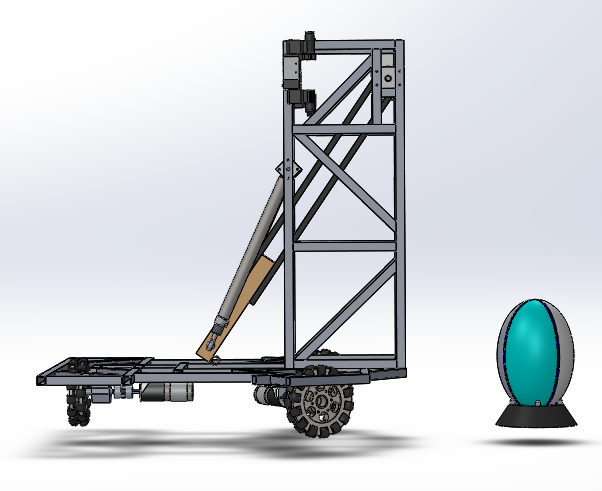
\includegraphics[scale=0.25]{Piston_kicking_1.PNG}} 
                    \captionof{figure}{Initial Positon.} \label{Piston_Kicking_1}
                \end{minipage}
                \hfil
                \begin{minipage}[b]{0.3\textwidth}
                    \frame{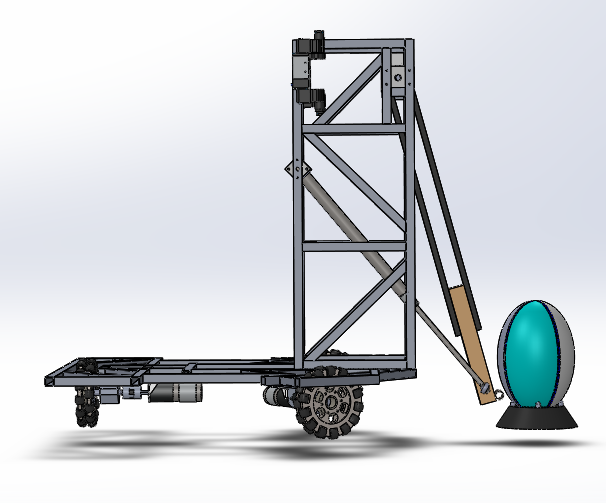
\includegraphics[scale=0.25]{Piston_kicking_2.PNG}} 
                    \captionof{figure}{Intermediate Positon.} \label{Piston_Kicking_2}
                \end{minipage}
                \hfil
                \begin{minipage}[b]{0.3\textwidth}
                    \frame{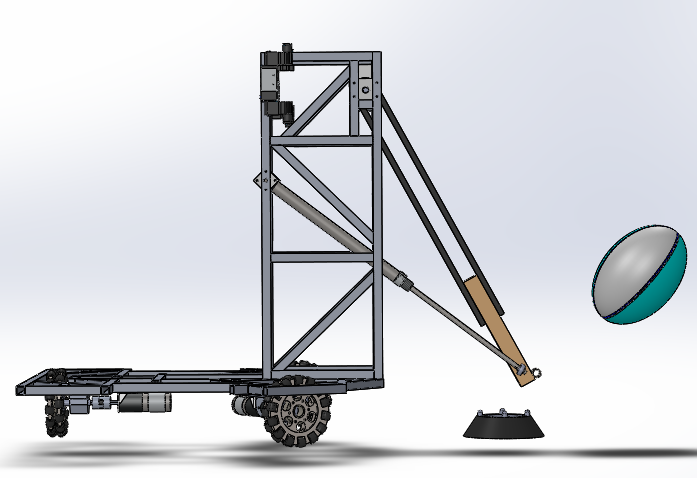
\includegraphics[scale=0.25]{Piston_kicking_3.PNG}} 
                    \captionof{figure}{Final Position} \label{Piston_Kicking_3}
                \end{minipage}                
            \end{minipage}         
%%%%%%%%%%%%%%%%%%%%%%%%%%%%%%%%%%%%%%%%%%%%%%%%%%%%%%%%%%%%%%%%%%%%%%%%%%%%%%%%%%%%%%%%%%%%%%%%%%%%%%%%%%%%%%%%%%%%%%%%%%%%%%%%%%%%%%%%%%%%
%%%%%%%%%%%%%%%%%%%%%%%%%%%%%%%%%%%%%%%%%%%%%%%%%%%%%%%%%%%%%%%%%% End %%%%%%%%%%%%%%%%%%%%%%%%%%%%%%%%%%%%%%%%%%%%%%%%%%%%%%%%%%%%%%%%%%%%%
%%%%%%%%%%%%%%%%%%%%%%%%%%%%%%%%%%%%%%%%%%%%%%%%%%%%%%%%%%%%%%%%%%%%%%%%%%%%%%%%%%%%%%%%%%%%%%%%%%%%%%%%%%%%%%%%%%%%%%%%%%%%%%%%%%%%%%%%%%%% 

%%%%%%%%%%%%%%%%%%%%%%%%%%%%%%%%%%%%%%%%%%%%%%%%%%%%%%%%%%%%%%%%%%%%%%%%%%%%%%%%%%%%%%%%%%%%%%%%%%%%%%%%%%%%%%%%%%%%%%%%%%%%%%%%%%%%%%%%%%%%
%%%%%%%%%%%%%%%%%%%%%%%%%%%%%%%%%%%%%%%%%%%%%%%%%%%%% End Of the Kicking Mechanism I %%%%%%%%%%%%%%%%%%%%%%%%%%%%%%%%%%%%%%%%%%%%%%%%%%%%%%%
%%%%%%%%%%%%%%%%%%%%%%%%%%%%%%%%%%%%%%%%%%%%%%%%%%%%%%%%%%%%%%%%%%%%%%%%%%%%%%%%%%%%%%%%%%%%%%%%%%%%%%%%%%%%%%%%%%%%%%%%%%%%%%%%%%%%%%%%%%%%



%%%%%%%%%%%%%%%%%%%%%%%%%%%%%%%%%%%%%%%%%%%%%%%%%%%%%%%%%%%%%%%%%%%%%%%%%%%%%%%%%%%%%%%%%%%%%%%%%%%%%%%%%%%%%%%%%%%%%%%%%%%%%%%%%%%%%%%%%%%%
%%%%%%%%%%%%%%%%%%%%%%%%%%%%%%%%%%%%%%%%%%%%%%%%%%%%% Start Of the Kicking Mechanism II %%%%%%%%%%%%%%%%%%%%%%%%%%%%%%%%%%%%%%%%%%%%%%%%%%%%%%%
%%%%%%%%%%%%%%%%%%%%%%%%%%%%%%%%%%%%%%%%%%%%%%%%%%%%%%%%%%%%%%%%%%%%%%%%%%%%%%%%%%%%%%%%%%%%%%%%%%%%%%%%%%%%%%%%%%%%%%%%%%%%%%%%%%%%%%%%%%%
    \subsection{Mechanism II}
    
        \subsubsection{Construction}
            The mechanism consists of a leg which is used as a hitting part for a kick ball. This leg is actuated using teo two PMDC motors 
            mounted coaxially and are opposite to each other.Two PMDC motors are mounted on a supported stucture which is made using 
            aluminium 6061 hollow square pipes to provide optimum strength to the mechanism.

%%%%%%%%%%%%%%%%%%%%%%%%%%%%%%%%%%%%%%%%%%%%%%%%%%%%%%%%%%%%%%%%%%%%%%%%%%%%%%%%%%%%%%%%%%%%%%%%%%%%%%%%%%%%%%%%%%%%%%%%%%%%%%%%%%%%%%%%%%%%
%%%%%%%%%%%%%%%%%%%%%%%%%%%%%%%%%%%%%%%%%%%%%%%% Design Calculation of the Motor Kicking %%%%%%%%%%%%%%%%%%%%%%%%%%%%%%%%%%%%%%%%%%%%%%%%%%
%%%%%%%%%%%%%%%%%%%%%%%%%%%%%%%%%%%%%%%%%%%%%%%%%%%%%%%%%%%%%%%%%%%%%%%%%%%%%%%%%%%%%%%%%%%%%%%%%%%%%%%%%%%%%%%%%%%%%%%%%%%%%%%%%%%%%%%%%%%%
        \subsubsection{Calculation}
            Initially, using Adams simulation software, the initial velocity that needs to be imparted to the ball so that it passes the
            conversion post from the desired distance was obtained. This velocity will be imparted to the ball through the impact of
            the leg. The leg should have a certain minimum velocity while the impact to achieve the desired results. This velocity
            will be provided by the motors.                                                                                                         \\
            To decide the torque and speed output required from the motor, the following energy conservation calculations were
            done.                                                                                                                                   \\   
            $$\frac{1}{2} I {\omega}^2  =  \frac{1}{2} m {\nu}^2$$     
            Where,                                                                                                                                  \\
            $I =$ Moment of Inertia of the leg;\tab $\omega =$ Angular speed of the leg.                                                            \\
            $\nu =$ Velocity of the ball;      \tab $m =$ Mass of the ball (340 g).                                                                 \\
            Based on the calculations, two motors of the following specifications are used                                                          \\
            •  RPM = 840 and Torque = 40 kg.cm                                                                                                      \\

%%%%%%%%%%%%%%%%%%%%%%%%%%%%%%%%%%%%%%%%%%%%%%%%%%%%%%%%%%%%%%%%%%%%%%%%%%%%%%%%%%%%%%%%%%%%%%%%%%%%%%%%%%%%%%%%%%%%%%%%%%%%%%%%%%%%%%%%%%%%
%%%%%%%%%%%%%%%%%%%%%%%%%%%%%%%%%%%%%%%%%%%%%%%%%%%%%%%%%%%%%%%%%% End %%%%%%%%%%%%%%%%%%%%%%%%%%%%%%%%%%%%%%%%%%%%%%%%%%%%%%%%%%%%%%%%%%%%%
%%%%%%%%%%%%%%%%%%%%%%%%%%%%%%%%%%%%%%%%%%%%%%%%%%%%%%%%%%%%%%%%%%%%%%%%%%%%%%%%%%%%%%%%%%%%%%%%%%%%%%%%%%%%%%%%%%%%%%%%%%%%%%%%%%%%%%%%%%%% 

%%%%%%%%%%%%%%%%%%%%%%%%%%%%%%%%%%%%%%%%%%%%%%%%%%%%%%%%%%%%%%%%%%%%%%%%%%%%%%%%%%%%%%%%%%%%%%%%%%%%%%%%%%%%%%%%%%%%%%%%%%%%%%%%%%%%%%%%%%%%%%
%%%%%%%%%%%%%%%%%%%%%%%%%%%%%%%%%%%%%%%%%%%%%%%%%%%% Working of the Kicking Mechanism II %%%%%%%%%%%%%%%%%%%%%%%%%%%%%%%%%%%%%%%%%%%%%%%%%%%%%%
%%%%%%%%%%%%%%%%%%%%%%%%%%%%%%%%%%%%%%%%%%%%%%%%%%%%%%%%%%%%%%%%%%%%%%%%%%%%%%%%%%%%%%%%%%%%%%%%%%%%%%%%%%%%%%%%%%%%%%%%%%%%%%%%%%%%%%%%%%%%%%

        \subsubsection{Working}       
            •  Ball Detection and Alignment:                                                                                                        \\
            The ball is detected using proximity and after detection ultrasonic sensor gives the distance of the ball from chassis,
            with the help of a lateral shifting robot is aligned for kicking.                                                                       \\
            •  Steps for Kicking:                                                                                                                   \\
            Motors are mounted on the top of the support structure and are connected to the Leg. 600 PPR rotary encoder is
            used for controlling the leg’s angular position. The kick is initialized by moving the leg vertically upwards making
            an angle of 180 degrees with respect to the structure. Then the motors are actuated, and this makes the leg rotate.
            Once the leg makes an impact with the ball, the power supply to the motors is ceased. But the leg continues to rotate
            due to its inertia.                                                                                                                     \\   

            \begin{minipage}[t]{\textwidth}
                \begin{minipage}[b]{0.3\textwidth}
                    \frame{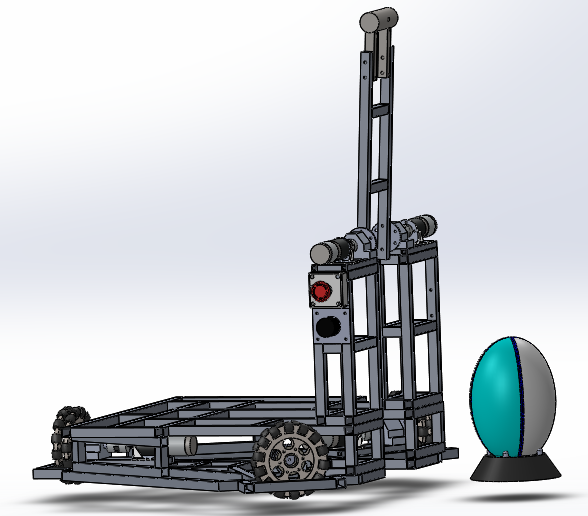
\includegraphics[scale=0.25]{Motor_kicking_1.PNG}} 
                    \captionof{figure}{Initial Positon.} \label{Motor_Kicking_1}
                \end{minipage}
                \hfil
                \begin{minipage}[b]{0.3\textwidth}
                    \frame{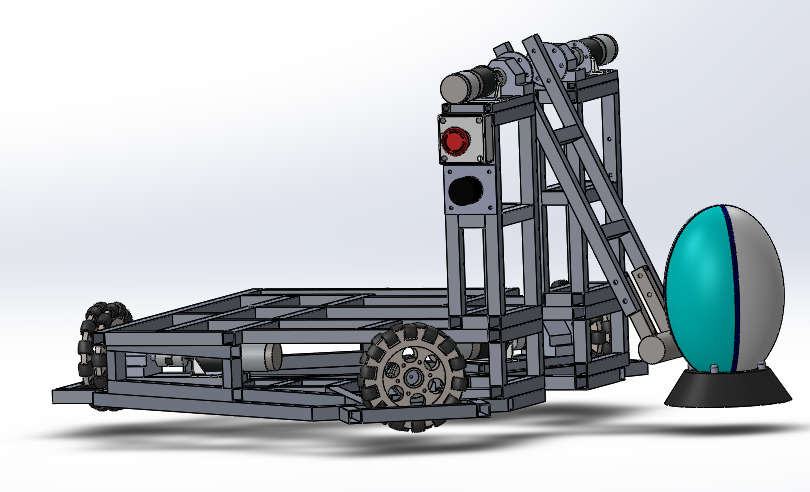
\includegraphics[scale=0.25]{Motor_kicking_2.PNG}} 
                    \captionof{figure}{Intermediate Positon.} \label{Motor_Kicking_2}
                \end{minipage}
                \hfil
                \begin{minipage}[b]{0.3\textwidth}
                    \frame{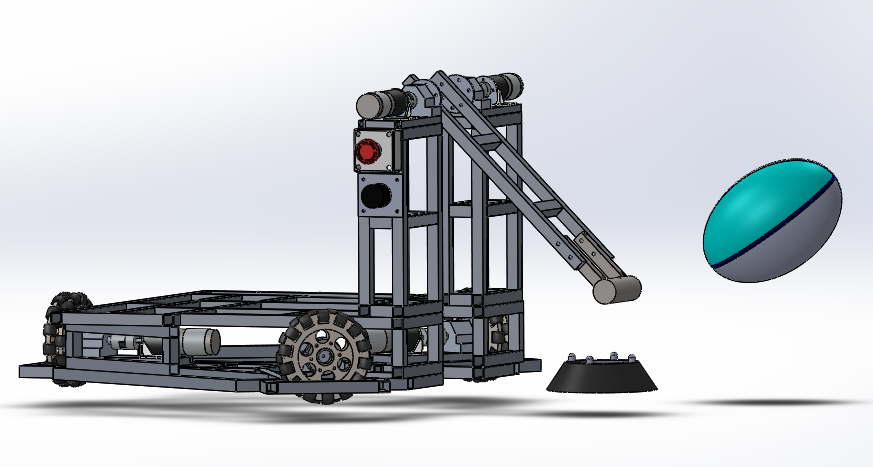
\includegraphics[scale=0.25]{Motor_kicking_3.PNG}} 
                    \captionof{figure}{Final Position} \label{Motor_Kicking_3}
                \end{minipage}                
            \end{minipage}   
%%%%%%%%%%%%%%%%%%%%%%%%%%%%%%%%%%%%%%%%%%%%%%%%%%%%%%%%%%%%%%%%%%%%%%%%%%%%%%%%%%%%%%%%%%%%%%%%%%%%%%%%%%%%%%%%%%%%%%%%%%%%%%%%%%%%%%%%%%%%
%%%%%%%%%%%%%%%%%%%%%%%%%%%%%%%%%%%%%%%%%%%%%%%%%%%%%%%%%%%%%%%%%% End %%%%%%%%%%%%%%%%%%%%%%%%%%%%%%%%%%%%%%%%%%%%%%%%%%%%%%%%%%%%%%%%%%%%%
%%%%%%%%%%%%%%%%%%%%%%%%%%%%%%%%%%%%%%%%%%%%%%%%%%%%%%%%%%%%%%%%%%%%%%%%%%%%%%%%%%%%%%%%%%%%%%%%%%%%%%%%%%%%%%%%%%%%%%%%%%%%%%%%%%%%%%%%%%%% 

%%%%%%%%%%%%%%%%%%%%%%%%%%%%%%%%%%%%%%%%%%%%%%%%%%%%%%%%%%%%%%%%%%%%%%%%%%%%%%%%%%%%%%%%%%%%%%%%%%%%%%%%%%%%%%%%%%%%%%%%%%%%%%%%%%%%%%%%%%%%
%%%%%%%%%%%%%%%%%%%%%%%%%%%%%%%%%%%%%%%%%%%%%%%%%%%%% End Of the Kicking Mechanism II %%%%%%%%%%%%%%%%%%%%%%%%%%%%%%%%%%%%%%%%%%%%%%%%%%%%%%
%%%%%%%%%%%%%%%%%%%%%%%%%%%%%%%%%%%%%%%%%%%%%%%%%%%%%%%%%%%%%%%%%%%%%%%%%%%%%%%%%%%%%%%%%%%%%%%%%%%%%%%%%%%%%%%%%%%%%%%%%%%%%%%%%%%%%%%%%%%%

%%%%%%%%%%%%%%%%%%%%%%%%%%%%%%%%%%%%%%%%%%%%%%%%%%%%%%%%%%%%%%%%%%%%%%%%%%%%%%%%%%%%%%%%%%%%%%%%%%%%%%%%%%%%%%%%%%%%%%%%%%%%%%%%%%%%%%%%%%%%
%%%%%%%%%%%%%%%%%%%%%%%%%%%%%%%%%%%%%%%%%%%%%%%%%%%%%%% End Of the Kicking Mechanism %%%%%%%%%%%%%%%%%%%%%%%%%%%%%%%%%%%%%%%%%%%%%%%%%%%%%%%
%%%%%%%%%%%%%%%%%%%%%%%%%%%%%%%%%%%%%%%%%%%%%%%%%%%%%%%%%%%%%%%%%%%%%%%%%%%%%%%%%%%%%%%%%%%%%%%%%%%%%%%%%%%%%%%%%%%%%%%%%%%%%%%%%%%%%%%%%%%%